\documentclass[aspectratio=169]{beamer}

\usetheme{Madrid}
\usecolortheme{seahorse}
\usefonttheme{professionalfonts}

\usepackage{listings}
\usepackage{xcolor}
\usepackage{tikz}
\usepackage{booktabs}
\usepackage{hyperref}
\usepackage{textcomp}
\usepackage{microtype}

\definecolor{codebg}{HTML}{1E1E2E}
\definecolor{codegreen}{HTML}{A6E3A1}
\definecolor{codeblue}{HTML}{89DCEB}
\definecolor{codeyellow}{HTML}{F9E2AF}
\definecolor{codegray}{HTML}{6C7086}
\definecolor{codepurple}{HTML}{CBA6F7}
\definecolor{codeorange}{HTML}{FAB387}
\definecolor{codewhite}{HTML}{CDD6F4}

\lstdefinestyle{clang}{
  backgroundcolor=\color{codebg},
  basicstyle=\ttfamily\footnotesize\color{codewhite},
  keywordstyle=\color{codepurple}\bfseries,
  commentstyle=\color{codegray}\itshape,
  stringstyle=\color{codegreen},
  numberstyle=\tiny\color{codegray},
  numbers=left, numbersep=6pt,
  breaklines=true, frame=single,
  rulecolor=\color{codeblue},
  language=C,
  tabsize=4
}

\title[MyOS Chapter 9]{\textbf{MyOS Chapter 9: Persistent Text Filesystem (PFS v1)}}
\subtitle{ATA-backed storage + create/write/read/hexdump/delete + reboot persistence}
\author{MyOS Project}
\date{March 2026}
\institute{x86 Protected Mode Kernel Engineering}

\newcommand{\concept}[2]{%
  \begin{block}{#1}\smallskip #2\smallskip\end{block}\vspace{5pt}}

\newcommand{\warn}[1]{%
  \begin{alertblock}{Important}\smallskip #1\smallskip\end{alertblock}\vspace{5pt}}

\begin{document}

\begin{frame}
  \titlepage
\end{frame}

\begin{frame}{Learning objectives}
  \begin{itemize}
    \item Understand the difference between in-memory files and persistent files
    \item Build a minimal block-backed filesystem with deterministic layout
    \item Implement end-user shell commands for full text-file lifecycle
    \item Diagnose and prevent common boot/storage integration failures
  \end{itemize}
  \concept{Scope of this chapter}{
    A practical persistent FS v1: single directory, fixed slots, text-friendly operations.
  }
\end{frame}

\begin{frame}{Why this chapter is a major milestone}
  \begin{itemize}
    \item RAMFS is useful for demos but data disappears after reboot
    \item Real OSes need storage decoupled from kernel binary image
    \item Persistent files unlock future executable loading and configuration persistence
    \item This chapter introduces your first true storage stack (driver + filesystem + shell API)
  \end{itemize}
\end{frame}

\begin{frame}{What was implemented end-to-end}
  \begin{itemize}
    \item ATA PIO disk I/O module: sector read/write via primary IDE ports
    \item PFS module: superblock + directory table + fixed data slots
    \item Automatic filesystem format on first valid boot (if metadata missing)
    \item Shell file commands: \texttt{ls}, \texttt{cat}, \texttt{hexdump}, \texttt{touch}, \texttt{write}, \texttt{rm}
    \item Persistent disk image attached in run pipeline: \texttt{build/data.img}
  \end{itemize}
\end{frame}

\begin{frame}{Storage stack architecture}
\begin{center}
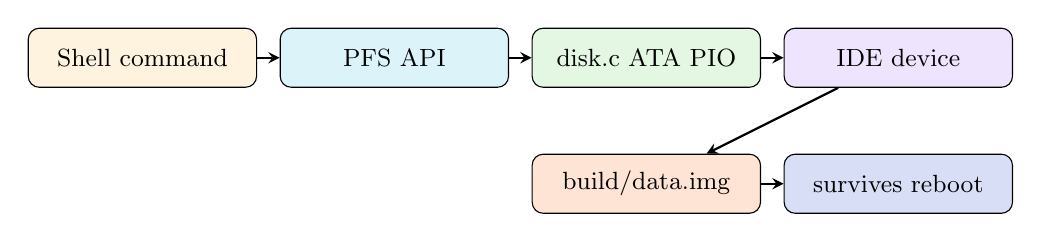
\begin{tikzpicture}[
  box/.style={rectangle,draw,rounded corners=4pt,
    minimum width=2.9cm,minimum height=0.75cm,
    align=center,font=\small},
  arr/.style={->,thick,>=stealth}]

  \node[box,fill=codeyellow!40] (shell) at (0,0) {Shell command};
  \node[box,fill=codeblue!30] (pfs) at (3.2,0) {PFS API};
  \node[box,fill=codegreen!30] (disk) at (6.4,0) {disk.c ATA PIO};
  \node[box,fill=codepurple!30] (ide) at (9.6,0) {IDE device};

  \node[box,fill=codeorange!35] (img) at (6.4,-1.6) {build/data.img};
  \node[box,fill=codewhite!80] (persist) at (9.6,-1.6) {survives reboot};

  \draw[arr] (shell) -- (pfs);
  \draw[arr] (pfs) -- (disk);
  \draw[arr] (disk) -- (ide);
  \draw[arr] (ide) -- (img);
  \draw[arr] (img) -- (persist);
\end{tikzpicture}
\end{center}
\end{frame}

\begin{frame}[fragile]{ATA PIO data path (kernel side)}
\begin{lstlisting}[style=clang]
int disk_read_sector(uint32_t lba, uint8_t* out_buffer) {
    ata_select_lba28(lba);
    outb(ATA_REG_COMMAND, ATA_CMD_READ_PIO);
    if (!ata_wait_ready()) return 0;

    for (int i = 0; i < 256; i++) {
        uint16_t w = inw(ATA_REG_DATA);
        out_buffer[i * 2]     = w & 0xFF;
        out_buffer[i * 2 + 1] = (w >> 8) & 0xFF;
    }
    return 1;
}
\end{lstlisting}
\concept{Engineering note}{
  Timeouts and not-busy checks are mandatory to avoid boot stalls when devices are absent or slow.
}
\end{frame}

\begin{frame}{PFS on-disk layout (v1)}
  \small
  \begin{tabular}{@{}p{3.4cm}p{8.6cm}@{}}
    \toprule
    \textbf{Region} & \textbf{Meaning} \\
    \midrule
    LBA 1 & Superblock (magic, version, max files, data start) \\
    LBA 2-3 & Directory table (32 entries total) \\
    LBA 4+ & File data sectors (one dedicated sector per file slot) \\
    \bottomrule
  \end{tabular}
  \vspace{6pt}
  \concept{Current limits}{
    32 files maximum, each file up to 480 bytes payload, single flat directory.
  }
\end{frame}

\begin{frame}[fragile]{Core PFS structures}
\begin{lstlisting}[style=clang]
typedef struct {
    uint32_t magic;
    uint32_t version;
    uint32_t max_files;
    uint32_t data_start_lba;
} pfs_superblock_t;

typedef struct {
    uint8_t used;
    char name[16];
    uint16_t size;
    uint32_t data_lba;
    uint8_t reserved[9];
} pfs_dir_entry_t;
\end{lstlisting}
\end{frame}

\begin{frame}[fragile]{Mount and auto-format strategy}
\begin{lstlisting}[style=clang]
void pfs_init() {
    read LBA1 into sector;
    if (magic/version/max_files invalid) {
        pfs_format_new();   // write clean superblock + empty dir + zero slots
    }
    g_ready = 1;
}
\end{lstlisting}
\concept{Why this is useful}{
  First boot requires no external formatter; filesystem self-initializes if unformatted.
}
\end{frame}

\begin{frame}{Shell command contract (user-facing API)}
  \small
  \begin{tabular}{@{}p{3.1cm}p{8.9cm}@{}}
    \toprule
    \textbf{Command} & \textbf{Behavior} \\
    \midrule
    \texttt{ls} & list persistent files and sizes \\
    \texttt{touch FILE} & create empty file (or keep existing with zero size write) \\
    \texttt{write FILE TEXT} & save text payload to file (overwrite, max 480 bytes) \\
    \texttt{cat FILE} & render printable content of persistent file \\
    \texttt{hexdump FILE} & inspect raw bytes in hex/ASCII view \\
    \texttt{rm FILE} & delete file entry and wipe its data sector \\
    \bottomrule
  \end{tabular}
\end{frame}

\begin{frame}[fragile]{Delete operation walkthrough}
\begin{lstlisting}[style=clang]
int pfs_delete_file(const char* name) {
    read_directory(dir);
    idx = find_file_index(dir, name);
    if (idx < 0) return 0;

    zero sector;
    disk_write_sector(dir[idx].data_lba, sector);  // wipe payload
    zero dir[idx];
    write_directory(dir);                           // remove metadata
    return 1;
}
\end{lstlisting}
\concept{Semantics}{
  Deletion removes discoverability and clears storage content in the file slot.
}
\end{frame}

\begin{frame}{Keyword glossary (storage layer)}
  \small
  \begin{tabular}{@{}p{3.0cm}p{9.0cm}@{}}
    \toprule
    \textbf{Keyword} & \textbf{Meaning} \\
    \midrule
    \texttt{ATA PIO} & CPU-driven IDE transfer mode using I/O ports and polling. \\
    \texttt{LBA} & Logical Block Address, sector index on block device. \\
    \texttt{superblock} & Filesystem metadata root (magic/version/layout). \\
    \texttt{directory entry} & Name + size + location metadata for one file. \\
    \texttt{slot} & Fixed storage unit reserved for one file in this v1 design. \\
    \texttt{persistence} & Data surviving emulator restarts and system reboots. \\
    \bottomrule
  \end{tabular}
\end{frame}

\begin{frame}{Keyword glossary (shell/data behavior)}
  \small
  \begin{tabular}{@{}p{3.0cm}p{9.0cm}@{}}
    \toprule
    \textbf{Keyword} & \textbf{Meaning} \\
    \midrule
    \texttt{overwrite} & New \texttt{write} replaces previous content of same file. \\
    \texttt{non-printable} & Byte outside visible ASCII range, shown as dot in text output. \\
    \texttt{hexdump} & Byte-level visualization for debugging and binary validation. \\
    \texttt{format-on-mount} & Automatic initialization when FS signature is absent/invalid. \\
    \texttt{flat namespace} & Single directory level; no subfolders in current version. \\
    \bottomrule
  \end{tabular}
\end{frame}

\begin{frame}{Integration changes by module}
  \small
  \begin{tabular}{@{}p{2.8cm}p{9.2cm}@{}}
    \toprule
    \textbf{Module} & \textbf{Change} \\
    \midrule
    \texttt{disk.c/h} & Added ATA LBA28 read/write sector operations with polling safeguards \\
    \texttt{pfs.c/h} & Added filesystem mount/list/read/write/delete APIs \\
    \texttt{kernel.c} & Added \texttt{pfs\_init()} in kernel boot path \\
    \texttt{shell.c} & Added file lifecycle commands and persistent backend routing \\
    \texttt{Makefile} & Added persistent disk image target and IDE drive attachment in QEMU run \\
    \bottomrule
  \end{tabular}
\end{frame}

\begin{frame}{Runtime validation protocol}
  \begin{enumerate}
    \item Boot and run \texttt{ls} (expect empty or existing persistent listing)
    \item Run \texttt{touch notes.txt}
    \item Run \texttt{write notes.txt Hello persistent world}
    \item Run \texttt{cat notes.txt}
    \item Run \texttt{hexdump notes.txt}
    \item Reboot and run \texttt{cat notes.txt} again (must persist)
    \item Run \texttt{rm notes.txt} and verify \texttt{ls} no longer shows it
  \end{enumerate}
\end{frame}

\begin{frame}{Failure modes and debugging guidance}
  \begin{itemize}
    \item \textbf{No shell prompt at boot}: likely kernel truncation due to fixed bootloader read budget
    \item \textbf{PFS not ready}: IDE disk not attached or ATA polling timeout/failure
    \item \textbf{write failed}: invalid name, full directory, oversized payload, or I/O failure
    \item \textbf{cat file not found}: missing file or directory metadata not committed
  \end{itemize}
  \warn{Bootloader sector budget must be revised as kernel grows, or runtime behavior appears random.}
\end{frame}

\begin{frame}{Security and robustness notes}
  \begin{itemize}
    \item No journaling or crash-consistency guarantees yet
    \item No checksums on superblock/directory entries
    \item No permission model or user separation
    \item Single-sector payload per file simplifies logic but limits growth
  \end{itemize}
  \concept{Why acceptable now}{
    This is a controlled educational stage focused on correctness of persistence pipeline.
  }
\end{frame}

\begin{frame}{Roadmap from PFS v1}
  \begin{itemize}
    \item Add \texttt{append}, \texttt{rename}, and file timestamps
    \item Support multi-sector extents per file and larger payloads
    \item Introduce allocation bitmap and free-space management
    \item Add a host-side image inspection and repair utility
    \item Integrate executable loader from persistent files
  \end{itemize}
\end{frame}

\begin{frame}{Outcome}
  \begin{itemize}
    \item MyOS now supports persistent text files across reboot cycles
    \item File lifecycle is complete in shell: create, write, read, inspect, delete
    \item Storage path is layered and testable (Shell -> PFS -> ATA -> Disk image)
    \item Kernel platform is now ready for executable loading from disk
  \end{itemize}
  \vspace{8pt}
  \begin{center}
    \Large \textbf{Chapter 9 establishes true persistent storage in MyOS.}
  \end{center}
\end{frame}

\end{document}
